\section{The \textsc{Platonis} platform}

\subsection{Architecture for mobile wireless applications}

In the first step, the \textsc{Platonis} network will not include a
corporate WAP gateway: we will use the operator gateway offered by
the industrial partner Kaptech. This architecture is shown in the
right part of the figure~\ref{fig:wap_network}. Three kinds of
terminal connection are provided: connection of a mobile phone
with WAP capability, connection of a PDA through a mobile phone
and direct connection of a PDA to the cellular network. The reader
will find details about terminal connections in
section~\ref{terminal_connection}.

Note that the network includes a Network Access Server(NAS), which 
is a gateway allowing the authentication of the terminals (client) 
before accessing the WAP gateway. 

The Kaptech operator will provide:

\begin{itemize}
\item a multi-gate access NAS (allowing to perform load tests);

\item an integration WAP gateway (with a secure access using
      \textsf{telnet} from the development stations of the platform)

\item an HTTP server demonstrator.

\end{itemize}

In the second step, the \textsc{Platonis} network will include a
corporate WAP gateway, allowing then protocol layer testing. 
The architecture is shown in the left part of the 
figure~\ref{fig:wap_network}. In this network each partner 
possesses his own development environment (more or less complete 
depending on their needs).  Note that it includes a \emph{Remote
Access Server} (RAS), which is a smaller version of NAS, before
accessing the WAP gateway.


\subsection{Connecting PDAs to wireless networks\label{terminal_connection}}

Recently there are a number of ways to connect a PDA to wireless 
network. In this section, we discuss various methods that are 
currently available for this connection. 
Figure~\ref{pda_connections} shows these configurations. 
\begin{figure}
\centering
\includegraphics[scale=0.5,bb=28 408 573 821]{pda_connections.eps}
\caption{Configurations for connecting PDAs to wireless networks
\label{pda_connections}}
\end{figure}
The methods can be mainly categorized into twofold: one is with aid of
a mobile phone and the other is without a mobile phone. If we have a
mobile phone, there are four configurations for connecting PDAs to
wireless networks, which depend on the availability of accessories and
the capability of the products.  If a mobile phone supports infrared
communication, PDAs can be connected to wireless networks through
infrared communication as shown in
figure~\ref{pda_connections}~(a). The advantages of this method are
that no other accessory is needed and that it can be applied to many
mobile phones and almost all PDAs since most of PDAs support infrared
communication.  However, the movement of the PDA and the mobile phone
is restricted during communication.  Otherwise the connection between
them may be lost. The second configuration is to use two serial
cables, each for a mobile phone and for a PDA as shown in
figure~\ref{pda_connections}~(b). The advantage of this method is that
it can be applied to many mobile phones. However, a few number of PDAs
have their serial cable for data communication and sometimes the
cables are bulky\footnote{Note that almost all PDAs have their serial
  cable for data synchronization with PC, not for data
  communication.}. The third configuration is to use one dedicated
cable for a mobile phone and PDA pair. In some cases the cable
accompanies a soft modem that is run on PDA. In other case the
dedicated cable is accompanied by a GSM modem card as is shown in
figure~\ref{pda_connections}~(d)\footnote{Soft modem and GSM modem
  cards are regular GSM modems.}.  The advantage of this configuration
is that it is lightweight.  It is also noted that the soft modem or
GSM modem provides better performance in wireless networks\footnote{We
  didn't check this yet.}. However, the mobile phone and PDA pairs
supported by this cable are restricted.

We can connect our PDAs to wireless networks without aid of 
mobile phones by using a GSM interface card where GSM modem 
is usually already built-in. Recently many companies have 
developed GSM interface cards for PDAs but not so many 
products are available yet. The advantage of this method is 
that we don't need mobile phones. In addition, we can usually make 
a phone call with this card using a software and a headset. The 
supported PDAs, however, are very restricted. 

If we consider the methods that will be available soon, we have 
more choices. A number of companies are developing a new product 
that is a combination of a mobile phone and a PDA. Some of them 
are already available now but not considered in this paper. A PDA 
can be connected to a mobile phone without any accessory if both 
of them support the Bluetooth technology. Some mobile phones 
already support the Bluetooth technology but currently no PDA 
supports it. Many PDA vendors are now integrating this technology 
to their PDAs.
